\begin{chapter}{Introduction}
\label{ch:introduction}

In this chapter we introduce the fundamental physical and mathematical ideas and
structures on which the other chapters build. The central objects here are the
time-dependent Schrödinger equation and a non-adiabatic potential.


\section{The time-dependent Schrödinger equation}

Time-dependent problems in quantum physics are governed by the time-dependent
Schrödinger equation:

\begin{equation} \label{eq:basics_tdse_simple}
  i \hbar \frac{\partial}{\partial t} \Ket{\varphi} = H \Ket{\varphi} \,.
\end{equation}

The Hamiltonian of the system in consideration is given by $H$, and the function
$\varphi\ofs{x,t}$ represents the wave function dependent on position $x$ and
time $t$. In $d$ space dimensions this is

\begin{align*}
  \varphi : \mathbb{R}^d \times \mathbb{R} & \rightarrow \mathbb{C} \\
                       \left( x, t \right) & \mapsto \varphi\ofs{x,t} \,.
\end{align*}

There are various mathematical restrictions on what is a valid wave-function. For
example $\varphi$ has to be square-integrable. Most of these preconditions have
little importance for us.

\section{Semiclassical scaling}

We use the semiclassical scaling, where $\varepsilon > 0$ is a real parameter
\footnote{Other authors use $\varepsilon$ or even $\hbar$ (without its physical
meaning and value) for the quantity we denote by $\varepsilon^2$.}. The equation
still keeps its mathematical form:

\begin{equation} \label{eq:basics_tdse_semi}
  i \varepsilon^2 \frac{\partial}{\partial t} \Ket{\psi} = H \Ket{\psi} \,.
\end{equation}

It's well known that we get the classical dynamics from the limit $\hbar \rightarrow 0$.
The same holds of course for the semiclassical parameter $\varepsilon$ and for bigger
$\varepsilon$ we get an increasing amount of quantum effects.

The Hamiltonian operator $H$ is composed of two parts, the kinetic operator $T$
and the potential operator $V$. Thus we can split $H$ as $H = T + V$ with the
following definitions for both operators. The mass $m$ which is present in the
common definition of the kinetic operator is included in the parameter $\varepsilon$.

\begin{equation} \label{eq:basics_def_ops}
\begin{split}
  T & \assign - \frac{1}{2} \varepsilon^4 \frac{\partial^2}{\partial x^2} \\
  V & \assign V\ofs{x}
\end{split}
\end{equation}

The potential is a real valued function depending only on space but not on time.
This static potential results from the Born-Oppenheimer approximation for
the electronic structure problem. For a more detailed theoretical background see
for example reference \cite{S_Teufel}. Assume the potential is given by:

\begin{equation} \label{eq:basics_potential_function}
\begin{split}
  V : \mathbb{R}^d & \rightarrow \mathbb{R} \\
                 x & \mapsto V\ofs{x}
\end{split}
\end{equation}

then this allows us to solve the Schrödinger equation by separation of variables
and obtain an analytical result for the time propagation of a quantum state $\Ket{\psi\ofs{t}}$

\begin{equation} \label{eq:basics_analytic_time_propagation}
  \Ket{\psi\ofs{t}} = e^{- \frac{i}{\varepsilon^2} H t } \Ket{\psi\ofs{0}} \,.
\end{equation}

The solutions to this time propagation have fine details. A typical wavepacket
is highly oscillatory with a wavelength $\bigO{\varepsilon^2}$ localised in space
with $\bigO{\varepsilon^2}$ and moving with a velocity of $\bigO{1}$. This tiny
structures are a challenge for the algorithms simulating them. We would need a very
fine grid and thus a huge bunch of grid nodes.


\section{Non-adiabatic potentials, avoided crossings}

Non-adiabatic potentials are potentials that consist of multiple energy levels.
These energy levels may intersect each other, but we are interested in a situation
that is called an \emph{avoided crossing}. That is, the two energy surfaces always
stay in a minimal distance. We call this distance the energy gap and denote it by
$\delta$. A very simple example of such an avoided crossing with only two energy
levels is shown in figure \ref{fig:example_avoided_crossing}.

\begin{figure}
  \centering
  \begin{asy}[width=\the\linewidth]
import graph;

real left = -2;
real right = 2;

real delta = 0.15;

real lambda0(real x) { return sqrt(tanh(x)^2+delta**2)/2; }
real lambda1(real x) { return -sqrt(tanh(x)^2+delta**2)/2; }

xaxis("$x$",Arrow);
yaxis("$y$",Arrow);

draw(graph(lambda0,left,right,operator ..),blue);
draw(graph(lambda1,left,right,operator ..),blue);

real u = lambda0(0);
real l = lambda1(0);

pair s = (0,l+0.05*delta);
pair e = (0,u-0.05*delta);

draw("$\delta$", s--e, red, Arrows, PenMargins);

real u = lambda0(2);
pair l1 = (1,u);

real u = lambda1(2);
pair l0 = (1,u);

label("$\lambda_1(x)$",l1+S);
label("$\lambda_0(x)$",l0+N);
\end{asy}

  \caption{Example of an avoided crossing of two energy levels.}
  \label{fig:example_avoided_crossing}
\end{figure}

Based on the class of physical potential in consideration we have a strict monotone
order of the eigenvalues for all $x$ in our space \footnote{This is a fairly strong
assumption that can be replaced by much weaker formulations more suitable for mathematical
analysis. But for our purpose it is sufficient and these details don't really matter.}.

\begin{equation}
  \lambda_0\ofs{x} > \lambda_1\ofs{x} > \ldots > \lambda_{N-1}\ofs{x} \qquad \forall x
\end{equation}

This global consistent order allows us to sort the eigenvalues and the corresponding
eigenvectors uniquely in decreasing order.

For a more elaborate study of the mathematical details and a classification of
different types of avoided crossings see reference \cite{H_classification}.

We are now interested what happens with an incoming wave-packet $\Ket{\psi}$ while
it traverses the narrow part. The magnitude $\delta$ of the energy gap plays an
important role in this process.

\section{A vector of states}

For the study of avoided crossings of the energy levels we are interested in vector valued
states $\Ket{\Psi}$. Each component of this vector represents a part of the wave function
being on the corresponding energy surface.

To describe the dynamics of these states, we need to generalize the Schrödinger equation
to a vector valued version. This is not difficult to do, basically the extended equation looks
exactly like \eqref{eq:basics_tdse_semi} but with the difference that $H$ is a matrix now.
Let's write down this in more detail because we will refer to it over and over again.

Assume we deal with $N$ different states hence $\Ket{\Psi}$ consists of $N$ components
$\varphi_i \ofs{x}$. And the Hamiltonian becomes a real valued symmetric $N \times N$
matrix. This gives the following expression for the time-dependent Schrödinger equation

\begin{equation} \label{eq:basics_tdse_vector}
  i \varepsilon^2 \frac{\partial}{\partial t} \Ket{ \begin{pmatrix}
                                                   \varphi_0 \\
                                                   \vdots \\
                                                   \varphi_{N-1}
                                                 \end{pmatrix}
                                               }
  =
  \begin{pmatrix}
    {} & {} & {} \\
    {} & H  & {} \\
    {} & {} & {} \\
  \end{pmatrix}
  \underbrace{
  \Ket{ \begin{pmatrix}
          \varphi_0 \\
          \vdots \\
          \varphi_{N-1}
        \end{pmatrix}
      }}_{\Ket{\Psi}} \,.
\end{equation}

\section{The potential}

In the case of a non-adiabatic potential with multiple energy levels,
the potential $V$ becomes a matrix. We assume that $V$ depends on space $x$
but not on time $t$, thus it is time-independent.

The matrix representing $V$ is symmetric and with entries $v_{i,j} \equiv v_{j,i} \in \mathbb{R}$. We may
write a general unspecified potential as

\begin{equation} \label{eq:general_potential_matrix}
  V\ofs{x} \rassign
  \begin{pmatrix}
    v_{0,0}\ofs{x} & \cdots & v_{0,N-1}\ofs{x} \\
    \vdots         &        & \vdots \\
    v_{N-1,0}\ofs{x} & \cdots & v_{N-1,N-1}\ofs{x}
  \end{pmatrix}
\end{equation}

where each of the matrix entries $v_{i,j}\ofs{x}$ is a real valued function

\begin{align*} \label{eq:matrix_potential_function_entry}
  v_{i,j} : \mathbb{R}^d & \rightarrow \mathbb{R} \\
                       x & \mapsto v_{i,j}\ofs{x}
\end{align*}

on its own. These functions are assumed to be smooth.

\subsection{Diagonalization of the potential}

We are much more interested in the potential's eigenvalues which are the energy
levels of our system. A well known result from linear algebra tells us that
symmetric matrices always have only real eigenvalues. Therefore we can diagonalize
this matrix and obtain pure real eigenvalues $\lambda_i\ofs{x}$ that depend on the
space variable $x$.

The diagonalization itself is performed by orthogonal matrices, the same theorem
as above guarantees that we have a full set of orthogonal eigenvectors $\nu_i\ofs{x}$
which depend of course on $x$ too.

Given the full set of eigenvalues $\lambda_0\ofs{x}, \ldots, \lambda_{N-1}\ofs{x}$
and the corresponding eigenvectors of $V\ofs{x}$ denoted by $\nu_0\ofs{x}, \ldots, \nu_{N-1}\ofs{x}$
the spectral decomposition of the potential's matrix reads

\begin{equation} \label{eq:general_spectral_transformation}
  \Lambda\ofs{x} = M^{-1}\ofs{x} V\ofs{x} M\ofs{x}
\end{equation}

where the matrix $\Lambda$ is diagonal with the eigenvalues $\lambda_i$ on its
diagonal. The transformation matrix $M$ is orthogonal and contains the
eigenvectors as columns:

\begin{equation} \label{eq:general_transformation_matirx}
  M \assign
  \begin{pmatrix}
    \nu_0\ofs{x} & , \hdots , & \nu_{N-1}\ofs{x}
  \end{pmatrix} \,.
\end{equation}

\subsubsection{The special case for 2 energy levels}

A general potential that only contains two energy levels is given by a symmetric
two by two matrix. In this case we can write down the eigenvalues for the potential
in closed form. The following formulae are defined in more detail in \cite{H_T_semiclassical_2x2}.
Suppose the potential matrix is given by

\begin{equation}
  V\ofs{x} \assign
  \begin{pmatrix}
    v_1 &  v_2 \\
    v_2 & -v_1
  \end{pmatrix}
\end{equation}

with trace $\text{Tr}\ofs{V} = 0$. Then we define a $\theta$ as

\begin{equation}
  \theta \assign \frac{1}{2} \arctan \ofs{\frac{v_2}{v_1}} \,.
\end{equation}

For the numerical computation we have to use the \texttt{atan2} function to get the signs
correct. Finally we can write the two eigenvectors as

\begin{equation}
  \nu_0 \assign
  \begin{pmatrix}
    \cos\ofs{\theta} \\
    \sin\ofs{\theta}
  \end{pmatrix}
  \quad
  \nu_1 \assign
  \begin{pmatrix}
    -\sin\ofs{\theta} \\
    \cos\ofs{\theta}
  \end{pmatrix} \,.
\end{equation}

Obviously they are orthogonal and normed. Remember that if we sort the $\lambda_i$
we have to change the order of the eigenvectors
as well. It's not guaranteed that $\nu_0$ always belongs to $\lambda_0$.

\subsection{Basis transformations of states}
\label{sec:basis_transformations_of_states}

For various calculations later on we need to be able to transform states from and to
the eigenbasis. This is in principle a trivial process of linear algebra, but lets
briefly note the important points.

The transformation from the eigenbasis to the canonical basis will be important
when we set up the initial values for a simulation. Assume we have a wave function
$\Ket{\varphi^e}$ given in the eigenbasis. The transformed state in the canonical
basis is given by

\begin{equation}
  \Ket{\varphi^c} = M \Ket{\varphi^e}
\end{equation}

where $M$ contains the column vectors $\nu_i$.

The opposite transformation becomes important when evaluating observables. Given
a state $\Ket{\varphi^c}$ in the canonical basis, the image of the transformation
into the eigenbasis is

\begin{equation}
  \Ket{\varphi^e} = M\T \Ket{\varphi^c}
\end{equation}

where we simplified $M^{-1} = M\T$ for real orthogonal matrices.

\section{The matrix exponential}

The exact time propagator for the Schrödinger equation is $e^{- \frac{i}{\varepsilon^2} H t }$
as shown in equation \eqref{eq:basics_tdse_semi}. If the Hamiltonian is matrix valued
then this expression becomes a matrix exponential. For that reason we need to
think about some aspects of this topic too.

\subsection{Symbolic matrix exponential}

Given a general $2 \times 2$ square matrix $M \in \mathbb{C}^{2 \times 2}$ we can derive
an analytical closed form expression for its exponential. We now try to find an
explicit formula for the exponential $\exp\ofs{M}$ of this matrix. For brevity
we just show the formula. A detailed derivation and the proof can be found in
reference \cite{matexp}.

Assume that our matrix looks like

\begin{equation}
  M \assign
  \begin{pmatrix}
    a & b\\
    c & d
  \end{pmatrix}
\end{equation}

with four possibly complex entries. Then

\begin{equation} \label{eq:symbolic_matrix_exp}
  e^M = e^{\frac{a + d}{2}}
  \begin{pmatrix}
    \cosh \left( \Delta \right) + \frac{a - d}{2}  \frac{\sinh \left( \Delta \right)}{\Delta} & b \frac{\sinh \left( \Delta \right)}{\Delta} \\
    c \frac{\sinh \left( \Delta \right)}{\Delta} & \cosh \left( \Delta \right) - \frac{a - d}{2}  \frac{\sinh \left( \Delta \right)}{\Delta}
  \end{pmatrix}
\end{equation}

where $\Delta$ is a discriminant of the form

\begin{equation}
  \Delta \assign \frac{1}{2} \sqrt{\left( a - d \right)^2 + 4 bc} \,.
\end{equation}

In the case of $\Delta=0$ we need to be careful because of a possible division by
zero and therefore consider a special case

\begin{equation}
e^M = e^{\frac{a + d}{2}}
  \begin{pmatrix}
    1 + \frac{a - d}{2} & b \\
    c & 1 - \frac{a - d}{2}
  \end{pmatrix} \,.
\end{equation}

\subsection{Numerical matrix exponential}

For matrices of size bigger than $2$ by $2$ there is no applicable symbolic expression
we could use. Hence the only possible solution is a numerical approximation. There
are many such approximations known in literature, see for example the excellent
survey of standard methods in reference \cite{moler_nineteen, moler_nineteen_later}.

In our implementation we just use the primitive function \texttt{expm} based on
Padé approximation available in scipy \cite{scipy}. But any other method like
for example Krylov methods can be used.

The general process of computing the matrix exponential of $V\ofs{x}$ numerically
for all grid nodes $\gamma$ is shown in figure \ref{fig:matrix_exponential_num}.
We start with evaluating the matrix $V$ of scalar functions at all grid nodes $\gamma$.
These values are stored in a suitable data structure. Then we slice this block
to get the matrix that belongs to a single node $\gamma_l$. The exponential of
this small $N \times N$ matrix is computed numerically, for example by \texttt{expm}.
After we did this for all grid nodes we can glue together all the exponentials
and arrive at a data structure identical to what we began with.

\begin{figure}[h]
  \centering
  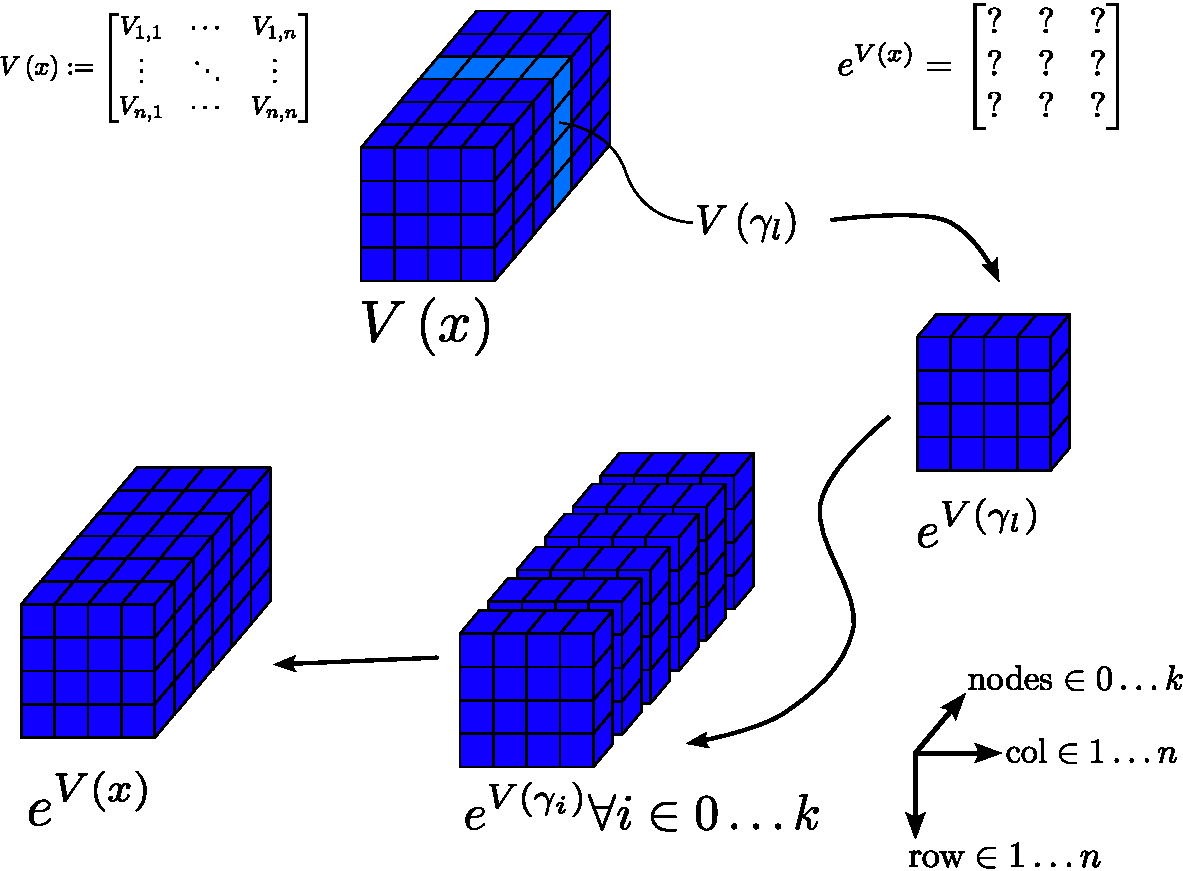
\includegraphics[width=0.8\linewidth]{./figures/matrix_exponential_num.pdf}
  \caption{Computation of the matrix exponential.}
  \label{fig:matrix_exponential_num}
\end{figure}


\end{chapter}